% ============================================================
%  IEEE TNSRE — Riemannian EEG Depression Detection
%  Main document file — structure only, content in sections/
% ============================================================
\documentclass[journal]{IEEEtran}
\IEEEoverridecommandlockouts

% ---------- Packages ----------
\usepackage{amsmath}
\usepackage{amssymb}
\usepackage{amsfonts}
\usepackage{graphicx}
\usepackage{xcolor}
\usepackage{tikz}
\usetikzlibrary{arrows.meta,calc,positioning,fit,backgrounds}
\newcommand{\hd}[1]{{\footnotesize\bfseries #1}}
\usepackage[colorlinks=true,linkcolor=blue,citecolor=blue,urlcolor=blue]{hyperref}
\usepackage[capitalise,noabbrev]{cleveref}
\usepackage{booktabs}
\usepackage{siunitx}
\usepackage[ruled,vlined,linesnumbered]{algorithm2e}
\usepackage{bm}
\usepackage{cite}

% ---------- Hyphenation hints ----------
\hyphenation{Rie-mann-ian co-var-i-ance MODMA LODO}

% ============================================================
\begin{document}

% ---------- Title ----------
\title{%
  SpectSPD-DANN: Riemannian Geometry and Adversarial SPD Alignment
  for Cross-Dataset EEG Depression Recognition%
}

% ---------- Authors ----------
% TODO: add all authors, affiliations, ORCID, corresponding author
\author{%
  % TODO: Replace with real author block
  Author One,~\IEEEmembership{Member,~IEEE,}
  Author Two,
  and~Author Three%
  \thanks{Manuscript received XXXX XX, 2026.}%
  \thanks{TODO: Add grant/funding acknowledgement here.}%
  \thanks{Corresponding author: TODO (email: TODO@institution.edu).}%
}

% Running headers
\markboth{IEEE Transactions on Neural Systems and Rehabilitation Engineering}%
{Author \MakeLowercase{\textit{et al.}}: SpectSPD-DANN for Cross-Dataset EEG Depression Recognition}

% ---------- Title page ----------
\maketitle

% ---------- Abstract ----------
\begin{abstract}
% TODO: Write abstract — MAX 250 words (TNSRE hard limit).
% Fill-in-the-blank template (from STYLE.md):
%   S1. Clinical scale: depression affects X; objective biomarkers needed.
%   S2. EEG + Riemannian geometry: covariance matrices on SPD manifold;
%       cite pennec2006riemannian, barachant2012multiclass.
%   S3. Gap: existing cross-dataset methods (e.g. WDANet) evaluate pairwise
%       source-to-target; Riemannian SPD geometry not applied to cross-dataset
%       depression transfer; no 3-way LODO benchmark exists.
%   S4. Method A (within-dataset): NrDE K=3 — transductive Riemannian K-NN +
%       DE spectral; 10-fold CV.
%   S5. Method B (cross-dataset): SpectSPD-DANN — SPD encoder + GRL domain
%       discriminator; 3-way LODO; 4-seed ensemble.
%   S6. Results: NrDE mean AUC 0.788 (3 datasets); competitive with EEG-RCformer
%       (0.7154) on MODMA. SpectSPD-DANN LODO mean AUC 0.723 (MODMA 0.764
%       >= WDANet 0.74-0.76 on harder 3-way protocol). Pooled N=232 AUC 0.788
%       Bal-Acc 0.710.
%   S7. Significance: demonstrates that optimal EEG depression model is
%       regime-dependent; provides the first 3-way LODO benchmark on three
%       independent EEG depression corpora under Riemannian geometry.
%   Write after Results section is complete.
ABSTRACT PLACEHOLDER — DO NOT SUBMIT.
\end{abstract}

% ---------- Keywords ----------
\begin{IEEEkeywords}
electroencephalography, depression detection, Riemannian geometry,
symmetric positive definite matrices, domain adaptation, transfer learning
\end{IEEEkeywords}

% ============================================================
%  Body — one file per section
% ============================================================
% ============================================================
%  Section: Introduction
%  Writing order: LAST (write after all other sections are done)
% ============================================================
\section{Introduction}
\label{sec:intro}
% TODO: Write introduction.
% Recommended paragraph structure:
%   P1 — Clinical motivation: burden of depression, under-diagnosis
%   P2 — EEG as a biomarker: non-invasive, neurophysiological correlates
%   P3 — Prior EEG depression work and the cross-subject gap
%   P4 — The cross-dataset (LODO) gap: why existing benchmarks are insufficient
%   P5 — Our contributions (bullet form):
%          (i) first strict LODO benchmark over N datasets
%          (ii) two-model framework: nrde K=3 within-dataset, SpecSPD-DANN cross-dataset
%          (iii) evidence that deep heads overfit at N~53 subjects
%   P6 — Paper organisation sentence

% Each paragraph should have a corresponding row in ../claims.csv before
% prose is drafted. See CLAUDE.md Rule 6.

% ============================================================
%  Section: Related Work
%  Writing order: THIRD (after Methods and Results)
% ============================================================
\section{Related Work}
\label{sec:related}
% TODO: Write related work.
% Recommended subsection structure:
%   \subsection{EEG Biomarkers of Depression}
%   \subsection{Riemannian Geometry for BCI and EEG Classification}
%   \subsection{Domain Adaptation for Cross-Subject EEG}
%   \subsection{Evaluation Protocols: Within-Subject vs.\ Cross-Dataset}
%
% For each cited work:
%   - State what they did in one sentence
%   - State the evaluation protocol used (within-subject / cross-subject / etc.)
%   - State why it is insufficient for the LODO setting we target
%
% Contrast table (optional): summarise prior work protocols in a table
% (dataset, N subjects, evaluation, method, reported metric)
%
% Each subsection paragraph must cite evidence from refs.bib.
% Unverified cites go in scripts/to-verify.txt (CLAUDE.md Rule 4).

% ============================================================
%  Section: Methodology
%  Claims: THESIS, BODY-002, BODY-003, BODY-004
%  Fixes: removed bold para-headers, all em-dashes, T=7680,
%         cohort, duplicate label, framing as one model
% ============================================================
\section{Methodology}
\label{sec:methods}

The proposed SpectSPD-DANN is a Riemannian geometry framework for EEG-based
depression detection that operates on the manifold of symmetric positive-definite
(SPD) matrices throughout the pipeline, from covariance estimation to
cross-dataset domain alignment.
Let $\mathcal{D}_k = \{(\mathbf{X}_{k,i},\,y_{k,i})\}_{i=1}^{N_k}$ denote the
$k$-th EEG dataset, where $\mathbf{X}_{k,i}\!\in\!\mathbb{R}^{p\times T}$ is a
multichannel segment with $p$ electrodes and $T$ samples (columns corresponding
to time points), and $y_{k,i}\!\in\!\{0,1\}$ indicates whether the subject belongs
to the MDD or HC group.
The corresponding SPD covariance representation is derived from
$\mathbf{X}_{k,i}$ in the processing stages described below.
Depending on the available training data, SpectSPD-DANN operates in two modes
selected according to an empirically observed performance crossover as dataset
size increases: for single-dataset evaluation at clinical scale
($N\!\approx\!53$), a transductive Riemannian nearest-neighbour mode (NrDE)
is used; for cross-dataset transfer and pooled evaluation, the full deep
adversarial SPD encoder is engaged.

% ── Datasets ──────────────────────────────────────────────────────────────────
\subsection{Datasets}
\label{sec:datasets}

This study uses three publicly available resting-state EEG depression datasets.
All original studies were conducted under institutional review board oversight
with written informed consent; IRB details are reported in the respective
publications~\cite{cai2022modma,mumtaz2016mdd,cavanagh2021openneuro}.
% TODO before submission: insert the explicit IRB name and protocol number from
% each dataset paper, as required by TNSRE journal policy (CLAUDE.md).
Table~\ref{tab:datasets} summarises the study characteristics.

\begin{table}[!t]
  \renewcommand{\arraystretch}{1.2}
  \caption{EEG Depression Datasets}
  \label{tab:datasets}
  \centering
  \begin{tabular}{lccccc}
    \toprule
    \textbf{Dataset} & \textbf{$N$} & \textbf{MDD/HC} & \textbf{Ch.}
      & \textbf{$f_s$ (Hz)} & \textbf{Label} \\
    \midrule
    MODMA~\cite{cai2022modma}             & 53  & 24/29  & 128 & 1000 & Clinical \\
    Mumtaz~\cite{mumtaz2016mdd}           & 58  & 34/24  & 14  & 256  & Clinical \\
    OpenNeuro~\cite{cavanagh2021openneuro} & 121 & 42/79 & 64  & 256  & BDI $\!\geq\!14$ \\
    \midrule
    \textbf{Total} & \textbf{232} & \textbf{100/132} & --- & --- & --- \\
    \bottomrule
  \end{tabular}
\end{table}

OpenNeuro assigns labels based on BDI self-report scores (BDI $\geq 14$ indicates
MDD), whereas MODMA and Mumtaz use clinician-administered structured interviews,
introducing a labeling-protocol mismatch whose impact is analysed separately in
Section~\ref{sec:results}.
Cross-dataset evaluation uses leave-one-dataset-out (LODO): train on $K\!-\!1\!=\!2$
datasets, test on all subjects of the held-out $K$-th; with $K\!=\!3$, this yields
three LODO folds.
Within-dataset evaluation uses 10-fold subject-stratified cross-validation within
each $\mathcal{D}_k$; test subjects appear in no training fold.

% ── A. EEG Covariance Representation ─────────────────────────────────────────
\subsection{EEG Covariance Representation}
\label{sec:cov}

The pairwise statistical relationships between EEG channels, which partially
reflect functional interactions between cortical regions, are a recognised
biomarker for major depression: inter-hemispheric asymmetry and fronto-parietal
coherence changes have been reported consistently across
studies~\cite{hosseinifard2013classifying,acharya2018automated}.
A covariance matrix $\mathbf{C}\in\mathbb{R}^{p\times p}$ captures
second-order pairwise linear relationships between channels; treating it as a
geometric object on the SPD manifold, rather than vectorising it into a
$\frac{p(p+1)}{2}$-dimensional Euclidean representation, preserves
congruence-transform invariance that makes the features robust to between-session
amplitude scaling and electrode impedance variation.

Let $\mathbf{X}\in\mathbb{R}^{p\times T}$ denote a 30-second EEG epoch with
$p=17$ harmonised channels and columns corresponding to time samples.
The mean-centred sample covariance is
\begin{equation}
  \hat{\mathbf{C}} = \frac{1}{T-1}\,\mathbf{X}\mathbf{H}\mathbf{X}^\top,
  \label{eq:sample_cov}
\end{equation}
where $\mathbf{H} = \mathbf{I}_T - \frac{1}{T}\mathbf{1}_T\mathbf{1}_T^\top$
is the $T\times T$ centering matrix.
Although $T \gg p$ in this setting, shrinkage is applied to improve numerical
conditioning and robustness.
We use the Ledoit-Wolf analytic shrinkage estimator~\cite{ledoit2004wellconditioned},
which minimises the expected Frobenius loss to the true population covariance:
\begin{equation}
  \mathbf{C} = (1 - \rho)\,\hat{\mathbf{C}} + \rho\,\hat{\mu}\,\mathbf{I}_p,
  \quad \hat{\mu} = \frac{\mathrm{tr}(\hat{\mathbf{C}})}{p},
  \label{eq:lw}
\end{equation}
where $\rho\in[0,1]$ is the analytically optimal shrinkage coefficient and
$\hat{\mu}$ is the average channel variance used as the shrinkage target.
For the estimated $\rho>0$, this yields a strictly positive-definite matrix
$\mathbf{C}\succ\mathbf{0}$, a necessary precondition for Riemannian operations.

Depression alters EEG power and coherence differently across frequency bands.
The raw epoch is bandpass-filtered into $B=5$ commonly used EEG frequency bands:
$\delta$ (0.5--4\,Hz), $\theta$ (4--8\,Hz), $\alpha$ (8--13\,Hz),
$\beta$ (13--30\,Hz), and $\gamma$ (30--45\,Hz), following the protocol
of Barachant et al.~\cite{barachant2012multiclass}.
A separate regularised covariance $\mathbf{C}^{(b)}\in\mathcal{S}^{++}_p$
is estimated in each band $b\in\{1,\ldots,B\}$ via~\eqref{eq:lw}.
This band-specific representation captures frequency-resolved connectivity
structure that a broadband covariance would conflate.

Prior to covariance estimation, each recording is bandpass-filtered
(0.5--45\,Hz, 4th-order Butterworth, zero-phase), common-average referenced,
downsampled to 256\,Hz, and segmented into non-overlapping 30-second epochs.
Epochs with peak-to-peak artefacts exceeding $150\,\mu\mathrm{V}$ are discarded.
The 17-channel harmonised montage (Fp1, Fp2, F3, F4, C3, C4, P3, P4, O1, O2,
F7, F8, T3, T4, T5, T6, Fz), the maximal common 10-20 subset across all three
datasets, is applied before covariance estimation.
\label{sec:preprocessing}

% ── B. Geometry of the SPD Manifold ───────────────────────────────────────────
\subsection{Geometry of the SPD Manifold}
\label{sec:manifold}

\begin{figure}[!t]
  \centering
  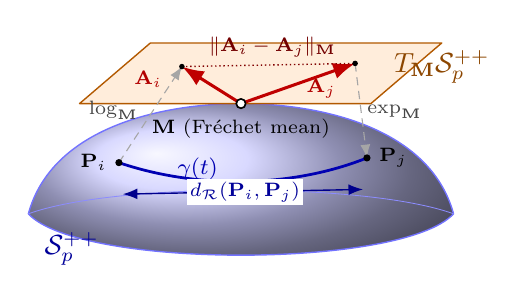
\begin{tikzpicture}[>=Latex,scale=1.0,line join=round]
    % ============ Manifold S_p^{++}: dome whose APEX is the tangency M ============
    \shade[ball color=blue!20,draw=blue!55,line width=0.5pt]
      (-2.7,0.15)
        .. controls (-2.4,1.25) and (-1.0,1.55) .. (0,1.55)
        .. controls (1.0,1.55) and (2.4,1.25) .. (2.7,0.15)
        .. controls (2.05,-0.55) and (-2.05,-0.55) .. (-2.7,0.15) -- cycle;
    \draw[blue!45,line width=0.3pt]
      (-2.7,0.15) .. controls (-1.6,0.55) and (1.6,0.55) .. (2.7,0.15);
    \node[blue!60!black,font=\itshape] at (-2.15,-0.30) {$\mathcal{S}^{++}_p$};
    % ============ Tangent plane, tangent to the dome exactly at M ============
    \fill[orange!14,draw=orange!70!black,line width=0.5pt]
      (-2.05,1.55) -- (1.65,1.55) -- (2.55,2.32) -- (-1.15,2.32) -- cycle;
    \node[orange!55!black,font=\itshape] at (2.55,2.02)
      {$T_{\mathbf{M}}\mathcal{S}^{++}_p$};
    % ============ Points ============
    \coordinate (M)  at (0,1.55);
    \coordinate (Pi) at (-1.55,0.80);
    \coordinate (Pj) at (1.60,0.86);
    \coordinate (Ai) at (-0.75,2.02);
    \coordinate (Aj) at (1.45,2.06);
    % ============ Geodesic gamma(t) on the manifold ============
    \draw[blue!70!black,line width=1.0pt]
      (Pi) .. controls (-0.55,0.46) and (0.65,0.48) .. (Pj);
    \node[blue!70!black,font=\footnotesize] at (-0.55,0.72) {$\gamma(t)$};
    \draw[<->,blue!55!black,line width=0.5pt] (-1.5,0.40) -- (1.55,0.46);
    \node[blue!60!black,font=\scriptsize,fill=white,inner sep=1pt] at (0.05,0.43)
      {$d_{\mathcal{R}}(\mathbf{P}_i,\mathbf{P}_j)$};
    % ============ Mapping arrows (directional) ============
    \draw[->,densely dashed,gray!70] (Pi) -- (Ai);
    \node[gray!55!black,font=\scriptsize] at (-1.62,1.46) {$\log_{\mathbf{M}}$};
    \draw[->,densely dashed,gray!70] (Aj) -- (Pj);
    \node[gray!55!black,font=\scriptsize] at (1.95,1.45) {$\exp_{\mathbf{M}}$};
    % ============ Tangent VECTORS anchored at M ============
    \draw[->,red!75!black,line width=1.1pt] (M) -- (Ai);
    \node[red!70!black,font=\scriptsize] at (-1.18,1.86) {$\mathbf{A}_i$};
    \draw[->,red!75!black,line width=1.1pt] (M) -- (Aj);
    \node[red!70!black,font=\scriptsize] at (1.02,1.74) {$\mathbf{A}_j$};
    \draw[densely dotted,red!50!black,line width=0.5pt] (Ai) -- (Aj);
    \node[red!45!black,font=\scriptsize] at (0.40,2.27)
      {$\|\mathbf{A}_i-\mathbf{A}_j\|_{\mathbf{M}}$};
    % ============ Markers ============
    \fill[black] (Pi) circle (1.3pt); \node[font=\scriptsize,left=1pt]  at (Pi) {$\mathbf{P}_i$};
    \fill[black] (Pj) circle (1.3pt); \node[font=\scriptsize,right=1pt] at (Pj) {$\mathbf{P}_j$};
    \fill[black] (Ai) circle (1.0pt);
    \fill[black] (Aj) circle (1.0pt);
    \draw[black,fill=white,line width=0.6pt] (M) circle (1.7pt);
    \node[font=\scriptsize,below=2pt] at (M) {$\mathbf{M}$ (Fr\'echet mean)};
  \end{tikzpicture}
  \caption{Geometry of the SPD manifold $\mathcal{S}^{++}_p$. Two covariance
  matrices $\mathbf{P}_i,\mathbf{P}_j$ lie on the curved manifold and are joined
  by the geodesic $\gamma(t)$, whose length is the affine-invariant Riemannian
  distance $d_\mathcal{R}(\mathbf{P}_i,\mathbf{P}_j)$~\eqref{eq:airm_dist}. The
  tangent space $T_{\mathbf{M}}\mathcal{S}^{++}_p$ is attached to the manifold at
  the Fréchet mean $\mathbf{M}$, which serves as the origin of the tangent space.
  The logarithmic map~\eqref{eq:log_map} maps each point to a tangent vector
  anchored at $\mathbf{M}$,
  $\mathbf{A}_i=\mathrm{Log}_{\mathbf{M}}(\mathbf{P}_i)$ and
  $\mathbf{A}_j=\mathrm{Log}_{\mathbf{M}}(\mathbf{P}_j)$; the exponential
  map~\eqref{eq:exp_map} is its inverse in a neighbourhood of $\mathbf{M}$. Once
  in the flat tangent space, points are compared by the Euclidean norm
  $\|\mathbf{A}_i-\mathbf{A}_j\|_{\mathbf{M}}$, which agrees with
  $d_\mathcal{R}$ to first order near $\mathbf{M}$ and enables standard vector
  operations on the resulting features.}
  \label{fig:manifold}
\end{figure}

Covariance matrices are not general real matrices: they must be symmetric and
positive definite.
Although $\mathcal{S}^{++}_p$ is an open subset of $\mathrm{Sym}_p$, the vector
space of $p\times p$ symmetric matrices, its natural geometry is
non-Euclidean~\cite{pennec2006riemannian,bhatia2009positive}.
Performing Euclidean operations on this space, such as computing the arithmetic
mean or measuring proximity by Frobenius norm, ignores the intrinsic manifold
geometry and may lead to distorted statistical estimates; Euclidean interpolation
does not follow geodesics and can distort distances and averages.
Riemannian geometry provides intrinsic distance, tangent vectors, and geodesics
that respect the positive-definite structure, as illustrated in
Fig.~\ref{fig:manifold}.

The SPD manifold of order $p$ is defined as
\begin{equation}
  \mathcal{S}^{++}_p = \bigl\{\mathbf{C}\in\mathbb{R}^{p\times p}
    : \mathbf{C} = \mathbf{C}^\top,\;
    \mathbf{v}^\top\mathbf{C}\mathbf{v} > 0\;
    \forall\,\mathbf{v}\in\mathbb{R}^p\setminus\{\mathbf{0}\}\bigr\}.
  \label{eq:spd_def}
\end{equation}
$\mathcal{S}^{++}_p$ is open in $\mathrm{Sym}_p$ with respect to the topology
induced on $\mathrm{Sym}_p$ (it is not open in $\mathbb{R}^{p\times p}$), and is
therefore a smooth manifold of dimension $\tfrac{p(p+1)}{2}$.
At each point $\mathbf{P}\in\mathcal{S}^{++}_p$, the tangent space is identified
with $T_\mathbf{P}\mathcal{S}^{++}_p = \mathrm{Sym}_p$~\cite{absil2008optimization}.

The manifold is endowed with the affine-invariant Riemannian metric
(AIRM)~\cite{pennec2006riemannian}, whose inner product at $\mathbf{P}$ is
\begin{equation}
  \langle \mathbf{U}, \mathbf{V}\rangle_\mathbf{P}
    = \mathrm{tr}\!\bigl(\mathbf{P}^{-1}\mathbf{U}\,\mathbf{P}^{-1}\mathbf{V}\bigr),
    \quad \mathbf{U},\mathbf{V}\in T_\mathbf{P}\mathcal{S}^{++}_p.
  \label{eq:airm_inner}
\end{equation}
The induced norm on the tangent space is
$\|\mathbf{S}\|_\mathbf{P} = \sqrt{\langle\mathbf{S},\mathbf{S}\rangle_\mathbf{P}}
= \sqrt{\mathrm{tr}(\mathbf{P}^{-1}\mathbf{S}\mathbf{P}^{-1}\mathbf{S})}$
for $\mathbf{S}\in T_\mathbf{P}\mathcal{S}^{++}_p$.
The geodesic distance induced by the AIRM between
$\mathbf{A}, \mathbf{B}\in\mathcal{S}^{++}_p$ is
\begin{equation}
  d_\mathcal{R}(\mathbf{A},\mathbf{B})
    = \bigl\|\mathrm{logm}\bigl(\mathbf{A}^{-\frac{1}{2}}\mathbf{B}
        \mathbf{A}^{-\frac{1}{2}}\bigr)\bigr\|_F
    = \sqrt{\sum_{i=1}^{p}\log^2\!\lambda_i(\mathbf{A}^{-1}\mathbf{B})},
  \label{eq:airm_dist}
\end{equation}
where $\mathrm{logm}(\cdot)$ is the principal matrix logarithm,
$\|\cdot\|_F$ is the Frobenius norm, and $\lambda_i(\mathbf{A}^{-1}\mathbf{B})$
denotes the $i$-th eigenvalue of $\mathbf{A}^{-1}\mathbf{B}$, equivalently the
generalised eigenvalues of the pair $(\mathbf{B},\mathbf{A})$ solving
$\mathbf{B}\mathbf{v}=\lambda\mathbf{A}\mathbf{v}$.
Although $\mathbf{A}^{-1}\mathbf{B}$ is generally non-symmetric, it is similar to
the SPD matrix $\mathbf{A}^{-1/2}\mathbf{B}\mathbf{A}^{-1/2}$, so its eigenvalues
are real and strictly positive and the logarithm in~\eqref{eq:airm_dist} is
well defined.
The AIRM is invariant under congruence transformations
$(\mathbf{A},\mathbf{B})\mapsto(\mathbf{W}\mathbf{A}\mathbf{W}^\top,
\mathbf{W}\mathbf{B}\mathbf{W}^\top)$ for any invertible
$\mathbf{W}$~\cite{pennec2006riemannian}, making the metric insensitive to
invertible linear reparameterizations of the signal space. In the EEG setting,
per-channel gain and session-level amplitude scaling correspond to diagonal
choices of $\mathbf{W}$ and are thus special cases of this
invariance~\cite{barachant2012multiclass}.

For $\mathbf{P},\mathbf{Q}\in\mathcal{S}^{++}_p$, the unique AIRM geodesic
joining them is
\begin{equation}
  \gamma(t) = \mathbf{P}^{\frac{1}{2}}
    \bigl(\mathbf{P}^{-\frac{1}{2}}\mathbf{Q}\mathbf{P}^{-\frac{1}{2}}\bigr)^{t}
    \mathbf{P}^{\frac{1}{2}},
  \quad t\in[0,1],
  \label{eq:geodesic}
\end{equation}
with $\gamma(0)=\mathbf{P}$ and $\gamma(1)=\mathbf{Q}$~\cite{bhatia2009positive}.
The exponential map $\mathrm{Exp}_\mathbf{P}:T_\mathbf{P}\mathcal{S}^{++}_p
\to\mathcal{S}^{++}_p$ maps a tangent vector $\mathbf{S}$ to a manifold point
by following this geodesic from $\mathbf{P}$ in direction $\mathbf{S}$:
\begin{equation}
  \mathrm{Exp}_\mathbf{P}(\mathbf{S})
    = \mathbf{P}^{\frac{1}{2}}
        \mathrm{expm}\!\bigl(\mathbf{P}^{-\frac{1}{2}}\mathbf{S}\mathbf{P}^{-\frac{1}{2}}\bigr)
      \mathbf{P}^{\frac{1}{2}}.
  \label{eq:exp_map}
\end{equation}
Its inverse, the logarithmic map
$\mathrm{Log}_\mathbf{P}:\mathcal{S}^{++}_p\to T_\mathbf{P}\mathcal{S}^{++}_p$,
maps a second SPD matrix $\mathbf{Q}\in\mathcal{S}^{++}_p$ back to the tangent
space and is
\begin{equation}
  \mathrm{Log}_\mathbf{P}(\mathbf{Q})
    = \mathbf{P}^{\frac{1}{2}}
        \mathrm{logm}\!\bigl(\mathbf{P}^{-\frac{1}{2}}\mathbf{Q}\mathbf{P}^{-\frac{1}{2}}\bigr)
      \mathbf{P}^{\frac{1}{2}},
  \label{eq:log_map}
\end{equation}
and satisfies $d_\mathcal{R}(\mathbf{P},\mathbf{Q})=\|\mathrm{Log}_\mathbf{P}(\mathbf{Q})\|_\mathbf{P}$~\cite{absil2008optimization}.
The pair $(\mathrm{Exp}_\mathbf{P},\mathrm{Log}_\mathbf{P})$ enables transfer of
manifold computations to a locally isometric Euclidean space.

The Frechet mean (Riemannian centre of mass) of a set
$\{\mathbf{C}_i\}_{i=1}^N\subset\mathcal{S}^{++}_p$ is
\begin{equation}
  \mathbf{M}^* = \underset{\mathbf{M}\in\mathcal{S}^{++}_p}{\arg\min}
    \sum_{i=1}^N d_\mathcal{R}^2(\mathbf{M},\mathbf{C}_i),
  \label{eq:frechet}
\end{equation}
which exists and is unique: $(\mathcal{S}^{++}_p, d_\mathcal{R})$ is a Hadamard
manifold (complete, simply connected, of non-positive sectional curvature), so
the squared-distance objective in~\eqref{eq:frechet} is geodesically convex and
admits a single
minimiser~\cite{karcher1977riemannian,bhatia2009positive}.
It is computed by the iterative Karcher mean update, a Riemannian gradient
descent on~\eqref{eq:frechet},
\begin{equation}
  \mathbf{M}_{k+1} = \mathrm{Exp}_{\mathbf{M}_k}\!
    \Bigl(\frac{1}{N}\sum_{i=1}^N \mathrm{Log}_{\mathbf{M}_k}(\mathbf{C}_i)\Bigr),
  \label{eq:karcher}
\end{equation}
which converges to the unique Fréchet mean; a few iterations suffice in
practice~\cite{boumal2023introduction}.

% ── C. Riemannian Feature Extraction ─────────────────────────────────────────
\subsection{Riemannian Feature Extraction}
\label{sec:features}

The logarithmic map at the Frechet mean $\mathbf{M}^*$ provides a locally
isometric embedding of $\mathcal{S}^{++}_p$ into the flat tangent space
$T_{\mathbf{M}^*}\mathcal{S}^{++}_p \cong \mathrm{Sym}_p$.
Choosing $\mathbf{M}^*$ as the expansion point minimises the average
linearisation error across the training set, yielding the most faithful
Euclidean approximation to the local Riemannian geometry of the
data~\cite{arsigny2006logeuclidean,bleuz2022tangent}.

Given the per-band Frechet mean $\mathbf{M}^{(b)*}$ computed from
training-fold covariance matrices $\{\mathbf{C}^{(b)}_i\}_{i\in\mathcal{I}_\mathrm{train}}$
via~\eqref{eq:karcher}, each covariance $\mathbf{C}^{(b)}$ is mapped to a
symmetric tangent matrix:
\begin{equation}
  \mathbf{S}^{(b)} = \mathrm{Log}_{\mathbf{M}^{(b)*}}\!\bigl(\mathbf{C}^{(b)}\bigr)
    = {\mathbf{M}^{(b)*}}^{\!\frac{1}{2}}
        \mathrm{logm}\!\bigl({\mathbf{M}^{(b)*}}^{\!-\frac{1}{2}}
          \mathbf{C}^{(b)}\,{\mathbf{M}^{(b)*}}^{\!-\frac{1}{2}}\bigr)
      {\mathbf{M}^{(b)*}}^{\!\frac{1}{2}}.
  \label{eq:tangent_proj}
\end{equation}
The upper triangle (including diagonal) of $\mathbf{S}^{(b)}$ is vectorised to
\begin{equation}
  \mathbf{s}^{(b)} = \mathrm{vech}\!\bigl(\mathbf{S}^{(b)}\bigr)
    \in \mathbb{R}^{p(p+1)/2},
  \label{eq:vech}
\end{equation}
where $\mathrm{vech}(\cdot)$ stacks the upper-triangular entries column by column.
With $p=17$, each band yields a 153-dimensional descriptor.
The mean $\mathbf{M}^{(b)*}$ is computed on training data only and applied to
held-out test data without update, preventing data leakage.

To complement the spatial connectivity structure in $\mathbf{s}^{(b)}$, spectral
power information is incorporated via differential
entropy~\cite{duan2013differential}.
For band $b$, the differential entropy of a Gaussian with variance
$\hat{\sigma}_b^2$ is
\begin{equation}
  \mathrm{DE}^{(b)} = \frac{1}{2}\log\!\bigl(2\pi e\,\hat{\sigma}_b^2\bigr),
  \label{eq:de}
\end{equation}
where $\hat{\sigma}_b^2$ is the per-channel averaged band-filtered signal
variance.
The combined NrDE feature vector is
\begin{equation}
  \mathbf{f} = \bigl[\mathbf{s}^{(1)},\ldots,\mathbf{s}^{(B)},
    \mathrm{DE}^{(1)},\ldots,\mathrm{DE}^{(B)}\bigr]
    \in \mathbb{R}^{B\cdot\frac{p(p+1)}{2} + B},
  \label{eq:nrde_feat}
\end{equation}
yielding a 770-dimensional representation per epoch ($B=5$, $p=17$:
$5\!\times\!153\!+\!5\!=\!770$).

For within-dataset evaluation, SpectSPD-DANN operates in its transductive
Riemannian nearest-neighbour mode.
Rather than training a global classifier on all subjects, for each test window
with per-band covariances $\{\mathbf{C}^{(b)}_\mathrm{test}\}_{b=1}^B$, all
training subjects $j\in\mathcal{I}_\mathrm{train}$ are ranked by their mean
Riemannian distance to the test point:
\begin{equation}
  r_j = \frac{1}{B}\sum_{b=1}^{B}
    d_\mathcal{R}\!\bigl(\mathbf{C}^{(b)}_\mathrm{test},\,
    \mathbf{M}^{(b)}_j\bigr),
  \label{eq:nrde_dist}
\end{equation}
where $\mathbf{M}^{(b)}_j$ is the Frechet mean of subject $j$'s per-band
covariance matrices.
The $K=3$ subjects with the smallest $r_j$ are selected, and a logistic
regression classifier ($\ell_2$-regularised, $C_{\mathrm{reg}}=1$) is fit on
their windows~\cite{barachant2010riemannian}.
This ensures the classifier is conditioned on subjects whose neural synchrony
geometry is maximally similar to the test subject.
$K=3$ was selected by a one-time sweep over $K\in\{1,2,3,4,5,8\}$ on a
held-out validation partition and frozen across all datasets and folds.

% ── D. Domain Adaptation on SPD Manifolds ─────────────────────────────────────
\subsection{Domain Adaptation on SPD Manifolds}
\label{sec:da}

When training on source dataset $\mathcal{D}_s$ and testing on target
$\mathcal{D}_t$, the EEG covariance distributions differ:
$P_s(\mathbf{C})\neq P_t(\mathbf{C})$ even when the class-conditional
distribution $P(y\mid\mathbf{C})$ is approximately invariant.
This covariate shift on $\mathcal{S}^{++}_p$ arises from hardware
differences, impedance variation, and inter-site demographic factors.
The shift manifests as a rotation of the principal axes of the covariance
distribution, not a simple location offset: re-centring at the Riemannian
mean corrects the first-order shift but leaves residual directional
misalignment that degrades classification.
Adversarial domain alignment is therefore preferred over re-centring
approaches~\cite{ganin2017dann}.

Let the source domain contain $N_s$ labelled windows
$\{(\mathbf{X}_i^s, y_i)\}_{i=1}^{N_s}$ and the target domain contain
$N_t$ unlabelled windows $\{\mathbf{X}_j^t\}_{j=1}^{N_t}$ from the held-out
dataset (transductive setting: target windows are present at training time, but
never their labels).
An encoder $F_e:\mathbb{R}^{p\times T}\to\mathbb{R}^d$, task classifier
$F_c:\mathbb{R}^d\to[0,1]$, and domain discriminator
$F_d:\mathbb{R}^d\to[0,1]$ are trained jointly as a min-max game:
\begin{equation}
  \min_{\theta_e,\theta_c}\max_{\theta_d}
    \;\mathcal{L}_\mathrm{cls}(\theta_e,\theta_c)
    \;-\;\lambda\,\mathcal{L}_\mathrm{dom}(\theta_e,\theta_d),
  \label{eq:minmax}
\end{equation}
where $\theta_e$, $\theta_c$, $\theta_d$ are the respective parameter sets
and $\lambda>0$ controls the trade-off between task accuracy and domain alignment.

% ── E. Proposed Network Architecture ─────────────────────────────────────────
\subsection{Proposed Network Architecture}
\label{sec:arch}

\begin{figure*}[!t]
  \centering
  \resizebox{\textwidth}{!}{%
  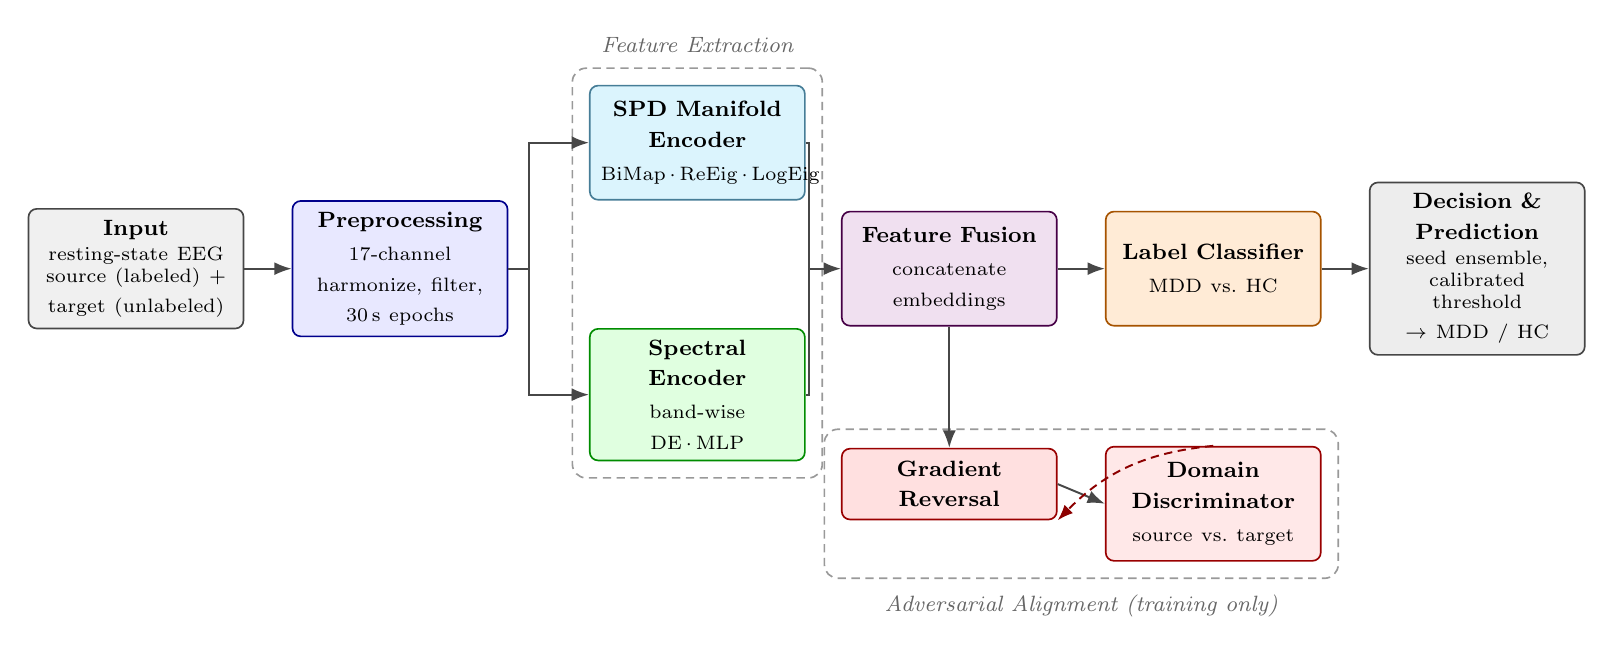
\begin{tikzpicture}[
    font=\small,
    base/.style={rounded corners=3pt, line width=0.6pt, align=center,
                 inner sep=4pt, draw=black!55, text width=2.45cm,
                 minimum height=1.45cm},
    arr/.style ={-{Latex[length=2.2mm]}, line width=0.7pt, draw=black!72},
    fl/.style  ={line width=0.7pt, draw=black!72},
    darr/.style={-{Latex[length=2.0mm]}, line width=0.7pt, draw=red!55!black,
                 densely dashed},
    grp/.style ={rounded corners=5pt, draw=black!40, densely dashed,
                 line width=0.6pt, inner sep=6pt},
    ttl/.style ={font=\footnotesize\itshape, black!60, align=center},
  ]
  % main horizontal spine
  \node[base, fill=gray!12, draw=gray!55!black] (in) at (0,0)
       {\hd{Input}\\[1pt]\scriptsize resting-state EEG\\ source (labeled) +\\ target (unlabeled)};
  \node[base, fill=blue!9, draw=blue!55!black, right=0.6cm of in] (pre)
       {\hd{Preprocessing}\\[1pt]\scriptsize 17-channel harmonize, filter, 30\,s epochs};
  % feature-extraction branches
  \node[base, fill=cyan!14, draw=cyan!55!black] at ($(pre.east)+(2.4,1.6)$) (spd)
       {\hd{SPD Manifold Encoder}\\[1pt]\scriptsize BiMap\,$\cdot$\,ReEig\,$\cdot$\,LogEig};
  \node[base, fill=green!12, draw=green!55!black] at ($(pre.east)+(2.4,-1.6)$) (spec)
       {\hd{Spectral Encoder}\\[1pt]\scriptsize band-wise DE\,$\cdot$\,MLP};
  \node[base, fill=violet!12, draw=violet!55!black] at ($(pre.east)+(5.6,0)$) (fuse)
       {\hd{Feature Fusion}\\[1pt]\scriptsize concatenate embeddings};
  \node[base, fill=orange!16, draw=orange!65!black, right=0.6cm of fuse] (cls)
       {\hd{Label Classifier}\\[1pt]\scriptsize MDD vs.\ HC};
  \node[base, fill=gray!14, draw=gray!55!black, right=0.6cm of cls] (out)
       {\hd{Decision \& Prediction}\\[1pt]\scriptsize seed ensemble,\\ calibrated threshold\\ $\rightarrow$ MDD / HC};
  % adversarial branch
  \node[base, fill=red!12, draw=red!60!black, minimum height=0.9cm] at ($(fuse.south)+(0,-2.0)$) (grl)
       {\hd{Gradient Reversal}};
  \node[base, fill=red!9, draw=red!60!black] at ($(cls.south)+(0,-2.25)$) (dom)
       {\hd{Domain Discriminator}\\[1pt]\scriptsize source vs.\ target};
  % arrows
  \coordinate (mrg) at ($(fuse.west)+(-0.4,0)$);
  \draw[arr] (in) -- (pre);
  \draw[arr] (pre.east) -- ++(0.26,0) |- (spd.west);
  \draw[arr] (pre.east) -- ++(0.26,0) |- (spec.west);
  \draw[fl]  (spd.east) -| (mrg);
  \draw[fl]  (spec.east) -| (mrg);
  \draw[arr] (mrg) -- (fuse.west);
  \draw[arr] (fuse) -- (cls);
  \draw[arr] (cls) -- (out);
  \draw[arr] (fuse.south) -- (grl.north);
  \draw[arr] (grl.east) -- (dom.west);
  \draw[darr] (dom.north) to[bend right=20] (grl.south east);
  % grouped containers
  \begin{scope}[on background layer]
    \node[grp, fit=(spd)(spec)] (fe) {};
    \node[grp, fit=(grl)(dom)]  (al) {};
  \end{scope}
  \node[ttl, above=2pt of fe.north] {Feature Extraction};
  \node[ttl, below=2pt of al.south] {Adversarial Alignment (training only)};
  \end{tikzpicture}%
  }
  \caption{Architecture of the proposed SpectSPD-DANN framework. Harmonized
  resting-state EEG from the labeled source corpora and the unlabeled held-out
  target corpus is encoded by two parallel branches: an SPD manifold encoder
  (covariance pooling followed by BiMap, ReEig, and LogEig layers) and a spectral
  encoder (band-wise differential entropy with an MLP). The fused representation
  feeds a label classifier trained on source labels and, through a gradient
  reversal layer, a domain discriminator that adversarially aligns the source and
  target distributions during training. At inference the discriminator branch is
  discarded; subject-level scores are combined by a seed ensemble and thresholded
  with a calibrated decision rule.}
  \label{fig:arch}
\end{figure*}

SpectSPD-DANN consists of two parallel feature streams, an SPD manifold
branch and a spectral DE branch, whose representations are fused before the
task classifier and the domain discriminator. Figure~\ref{fig:arch} illustrates
the complete architecture.

The SPD branch maps a raw EEG segment $\mathbf{X}\in\mathbb{R}^{p\times T}$
to a manifold-aware Euclidean embedding through four sequential stages.

\textit{Stage 1: Temporal convolution.}
A 1-D causal convolution with $n_f$ filters of length $\ell$ maps $\mathbf{X}$
to a hidden representation $\mathbf{H}\in\mathbb{R}^{p\times T'}$.
This step learns band-selective spatial filters jointly with the downstream SPD
objective, adapting to the depression-relevant frequency structure in the data.

\textit{Stage 2: Differentiable covariance pooling.}
A symmetric covariance pooling layer collapses the temporal axis:
\begin{equation}
  \mathbf{C}_0 = \frac{1}{T'}\,\mathbf{H}\mathbf{H}^\top
    \;\in\;\mathcal{S}^{+}_p.
  \label{eq:cov_pool}
\end{equation}
This differentiable operation, used in SPDNet-style
architectures~\cite{huang2017riemannian,cheng2026spd}, makes the branch
end-to-end trainable while operating in $\mathcal{S}^{++}_p$ from this stage
forward.

\textit{Stage 3: BiMap projection.}
The $p\times p$ SPD matrix $\mathbf{C}_0$ is projected to a lower-dimensional
$q\times q$ SPD matrix via a learnable congruence transformation:
\begin{equation}
  \mathbf{C}_1 = \phi_\mathbf{W}(\mathbf{C}_0) = \mathbf{W}\mathbf{C}_0\mathbf{W}^\top,
  \quad \mathbf{W}\in\mathbb{R}^{q\times p},\quad q = 12.
  \label{eq:bimap}
\end{equation}
If $\mathbf{W}$ has full row rank, then for any $\mathbf{v}\neq\mathbf{0}$,
$\mathbf{v}^\top\mathbf{C}_1\mathbf{v} = (\mathbf{W}^\top\mathbf{v})^\top
\mathbf{C}_0(\mathbf{W}^\top\mathbf{v}) > 0$, so
$\mathbf{C}_1\in\mathcal{S}^{++}_q$.
This BiMap layer, introduced in SPDNet~\cite{huang2017riemannian}, is the
canonical manifold-preserving dimensionality reduction on $\mathcal{S}^{++}$;
it reduces the $p\!=\!17$ covariance to a $q\!=\!12$ subspace that concentrates
the depression-relevant variance.

\textit{Stage 4: ReEig and LogEig.}
Gradient-based optimisation can drive eigenvalues of $\mathbf{C}_1$ toward zero,
violating strict positive definiteness.
The rectified eigenvalue (ReEig) layer~\cite{huang2017riemannian} floors all
eigenvalues at $\varepsilon$:
\begin{equation}
  \mathbf{C}_2 = \phi_\mathrm{rec}(\mathbf{C}_1)
    = \mathbf{U}\,\mathrm{diag}\!\bigl(\max(\lambda_1,\varepsilon),\ldots,
      \max(\lambda_q,\varepsilon)\bigr)\mathbf{U}^\top,
  \label{eq:reeig}
\end{equation}
where $\mathbf{C}_1 = \mathbf{U}\,\mathrm{diag}(\lambda_1,\ldots,\lambda_q)\,\mathbf{U}^\top$
is the eigendecomposition and $\varepsilon = 10^{-4}$.
The matrix logarithm (LogEig) layer then maps $\mathbf{C}_2$ to the tangent
space at the identity $\mathbf{I}_q$, following the log-Euclidean
framework~\cite{arsigny2007geometric}:
\begin{equation}
  \mathbf{Z} = \phi_\mathrm{log}(\mathbf{C}_2)
    = \mathrm{logm}(\mathbf{C}_2)
    = \mathbf{U}\,\mathrm{diag}(\log\lambda_1,\ldots,\log\lambda_q)\,\mathbf{U}^\top,
  \label{eq:logeig}
\end{equation}
vectorised to $\mathbf{z}_\mathrm{spd} = \mathrm{vech}(\mathbf{Z})
\in\mathbb{R}^{q(q+1)/2}$.
With $q=12$, the SPD branch produces a 78-dimensional output.
ReEig and LogEig have no learnable parameters; their Jacobians are computed
analytically for backpropagation through the
eigendecomposition~\cite{huang2017riemannian}.

The DE spectral features from~\eqref{eq:de} are computed over the same epoch
in the same $B=5$ bands and passed through a two-layer MLP with ReLU activations,
producing $\mathbf{z}_\mathrm{de}\in\mathbb{R}^{d_\mathrm{de}}$.
The two branch outputs are then concatenated to form the shared representation:
\begin{equation}
  \mathbf{h} = \bigl[\mathbf{z}_\mathrm{spd};\,\mathbf{z}_\mathrm{de}\bigr]
    \in \mathbb{R}^{d},\quad d = \tfrac{q(q+1)}{2} + d_\mathrm{de},
  \label{eq:fusion}
\end{equation}
which is passed to both the task head $F_c$ and the domain discriminator $F_d$.

% ── F. Training Objective and Optimization ────────────────────────────────────
\subsection{Training Objective and Optimization}
\label{sec:training}

The task head $F_c$ maps $\mathbf{h}$ to a probability
$\hat{p} = F_c(\mathbf{h})\in[0,1]$ via a fully connected layer with sigmoid
activation.
The binary cross-entropy over labelled source windows is
\begin{equation}
  \mathcal{L}_\mathrm{cls}(\theta_e,\theta_c)
    = -\frac{1}{N_s}\sum_{i=1}^{N_s}
        \bigl[y_i\log\hat{p}_i + (1-y_i)\log(1-\hat{p}_i)\bigr].
  \label{eq:cls_loss}
\end{equation}
The domain discriminator $F_d$ maps $\mathbf{h}$ to a domain label probability
$\hat{d}\in[0,1]$ ($d=0$: source; $d=1$: target), with cross-entropy
\begin{equation}
  \mathcal{L}_\mathrm{dom}(\theta_e,\theta_d)
    = -\frac{1}{N_s+N_t}\sum_{i=1}^{N_s+N_t}
        \bigl[d_i\log\hat{d}_i + (1-d_i)\log(1-\hat{d}_i)\bigr].
  \label{eq:dom_loss}
\end{equation}
The min-max problem~\eqref{eq:minmax} is solved with a single forward-backward
pass using a gradient reversal layer (GRL)~\cite{ganin2017dann} between $F_e$
and $F_d$.
In the forward pass the GRL acts as the identity; in the backward pass it scales
and negates the gradient flowing from $F_d$ to $F_e$:
\begin{equation}
  \frac{\partial\tilde{\mathcal{L}}}{\partial\mathbf{h}}
    = -\lambda\,\frac{\partial\mathcal{L}_\mathrm{dom}}{\partial\mathbf{h}}.
  \label{eq:grl}
\end{equation}
The encoder is thus trained to simultaneously minimise $\mathcal{L}_\mathrm{cls}$
and confuse the domain discriminator, yielding the joint objective:
\begin{equation}
  \mathcal{L} = \mathcal{L}_\mathrm{cls} - \lambda\,\mathcal{L}_\mathrm{dom}.
  \label{eq:joint_loss}
\end{equation}
The coupling coefficient $\lambda$ is annealed following the schedule
of Ganin et al.~\cite{ganin2017dann}:
$\lambda(t) = \frac{2}{1+\exp(-\gamma t/T_{\max})} - 1$, with $\gamma=10$.
All parameters are optimised jointly with Adam at learning rate $10^{-2}$ for
80 epochs, batch size 32.
The BiMap weight $\mathbf{W}$ is initialised from a truncated normal distribution
and regularised by its Frobenius norm to maintain full row rank.

Because the adversarial objective~\eqref{eq:joint_loss} is sensitive to
initialisation of $\theta_d$, four independent training runs are performed per
LODO fold with seeds $\mathcal{S}=\{42,1,2,3\}$.
Per-window prediction scores from each run are averaged at the subject level:
\begin{equation}
  \hat{p}_i^{\,\mathrm{ens}}
    = \frac{1}{|\mathcal{S}|}\sum_{s\in\mathcal{S}}\hat{p}_i^{(s)},
  \label{eq:ensemble}
\end{equation}
where $\hat{p}_i^{(s)}$ is the subject-level mean score from seed $s$.

% ── G. Inference Procedure ────────────────────────────────────────────────────
\subsection{Inference Procedure}
\label{sec:evaluation}

For within-dataset evaluation, each test subject's 30-second windows are
evaluated independently via~\eqref{eq:nrde_dist} and~\eqref{eq:nrde_feat}.
The $K=3$ nearest training subjects are located in Riemannian space, a logistic
classifier is fit on their windows, and per-window scores are averaged to obtain
a subject-level classification probability.
For cross-dataset evaluation, the trained encoder $F_e$ and task head $F_c$
are applied to all windows of the held-out target dataset, with subject-level
scores aggregated across seeds via~\eqref{eq:ensemble}.

A decision threshold $\tau^*$ is set by maximising balanced accuracy on the
training-fold subjects:
\begin{equation}
  \tau^* = \underset{\tau\in\mathbb{R}}{\arg\max}
    \;\mathrm{BAcc}\!\bigl(\{\hat{p}_i^{\,\mathrm{ens}}\}_{i\in\mathcal{I}_\mathrm{train}},\,\tau\bigr),
  \label{eq:thresh}
\end{equation}
where $\mathcal{I}_\mathrm{train}$ indexes training-fold subjects.
This threshold is then applied unchanged to the held-out test subjects.
Fitting $\tau^*$ on the test set itself inflates accuracy by an amount
proportional to the test set size and is explicitly avoided.

The primary metric is AUC (area under the ROC curve)~\cite{fawcett2006roc},
which measures $P(\hat{p}_\mathrm{MDD}>\hat{p}_\mathrm{HC})$, is threshold-free,
and is invariant to class imbalance.
Balanced accuracy and accuracy at $\tau^*$ are secondary.
Pairwise model comparisons use the Wilcoxon signed-rank test across $N=10$ CV
folds; all results follow the format: mean $\pm$ std ($p$-value; Wilcoxon
signed-rank; $N=10$ folds). Per-fold LODO values are reported individually.

% ============================================================
%  Section: Experimental Results
%  Writing order: SECOND (write after Methods)
% ============================================================
\section{Experimental Results}
\label{sec:results}
% TODO: Write results.
% Recommended subsection structure:
%
%   \subsection{Datasets}
%     - Table: dataset name, N subjects, channels, sampling rate, label balance
%     - MODMA: N~53, note small-N implication for deep networks
%     - Mumtaz / other datasets used
%
%   \subsection{Within-Dataset Performance (Nr\,DE, K=3)}
%     - Table: per-dataset AUC mean +/- std across LOSO folds
%     - Claims.csv entries: result claim for K=3 nrde AUC
%     - Ablation: K=1,2,3,5,10 AUC curve (if available)
%
%   \subsection{Cross-Dataset Performance (SpecSPD-DANN)}
%     - Table: source -> target AUC, mean +/- std, N folds
%     - Claims.csv entries: result claim for SpecSPD-DANN cross-dataset
%     - Seed stability analysis (3-5 seeds; report std across seeds)
%
%   \subsection{Ablation: Deep Heads vs.\ Riemannian Features}
%     - Motivation: deep networks overfit at N~53 (see claims.csv BG-003)
%     - Show AUC degradation with MLP/CNN heads on MODMA
%
%   \subsection{Comparison with Prior Work}
%     - Table: method, dataset, evaluation protocol, AUC/acc reported
%     - IMPORTANT: only compare methods using equivalent protocols
%       (no apples-to-oranges with within-subject results) — CLAUDE.md Rule 7
%
% Every numeric claim in this section MUST have a claims.csv row
% with evidence_file pointing to results/*.json or results/*.log.

% ============================================================
%  Section: Discussion
%  Writing order: FOURTH (after Results)
% ============================================================
\section{Discussion}
\label{sec:discussion}
% TODO: Write discussion.
% Recommended paragraph structure:
%
%   P1 — Summary of main finding: Riemannian features generalise; deep heads do not at N~53
%   P2 — Why K=3 works: geometric interpretation of nearest prototypes
%   P3 — SpecSPD-DANN: where it succeeds and fails (seed instability on Mumtaz-target)
%   P4 — The dataset-level shift problem: what LODO reveals that LOSO hides
%   P5 — Limitations:
%          - 17-channel harmonisation loses spatial resolution
%          - Binary classification (MDD vs. HC); does not handle severity
%          - SpecSPD-DANN seed instability on Mumtaz target (cite evidence)
%          - Small N in MODMA constrains deep model conclusions
%   P6 — Future directions: larger datasets, severity regression, online adaptation
%
% Do not use "delve", "leverage", "it is worth noting" — see CLAUDE.md AI-ism watchlist.
% Vary sentence length; avoid passive-voice-only paragraphs (CLAUDE.md Rules).

% ============================================================
%  Section: Conclusion
%  Writing order: FIFTH (after Discussion)
% ============================================================
\section{Conclusion}
\label{sec:conclusion}
% TODO: Write conclusion (~1 paragraph, ~150 words).
% Must cover:
%   - What we proposed (two-model Riemannian framework for LODO EEG depression)
%   - Key result (nrde K=3 AUC within-dataset; SpecSPD-DANN AUC cross-dataset)
%   - Key insight (Riemannian features + small-K prototype generalise; deep heads overfit)
%   - One-sentence forward look (larger cohort studies / clinical deployment)
%
% DO NOT begin with "In conclusion" — this is an IEEE-ism that reviewers flag.
% DO NOT copy from Abstract — paraphrase the contribution, not the methods.


% ---------- Acknowledgments ----------
\section*{Acknowledgments}
% TODO: funding, ethics approval, dataset access acknowledgements
ACKNOWLEDGMENTS PLACEHOLDER.

% ---------- References ----------
\bibliographystyle{IEEEtran}
\bibliography{refs}

% ---------- Biographies (optional for TNSRE) ----------
% TODO: add author bios when ready
% \begin{IEEEbiographynophoto}{Author One}
% Bio text here.
% \end{IEEEbiographynophoto}

\end{document}
